\chapter{研究方法}
\section{實驗環境與架構設計}
\begin{figure}[!htbp]
\centering
\scalebox{.35}{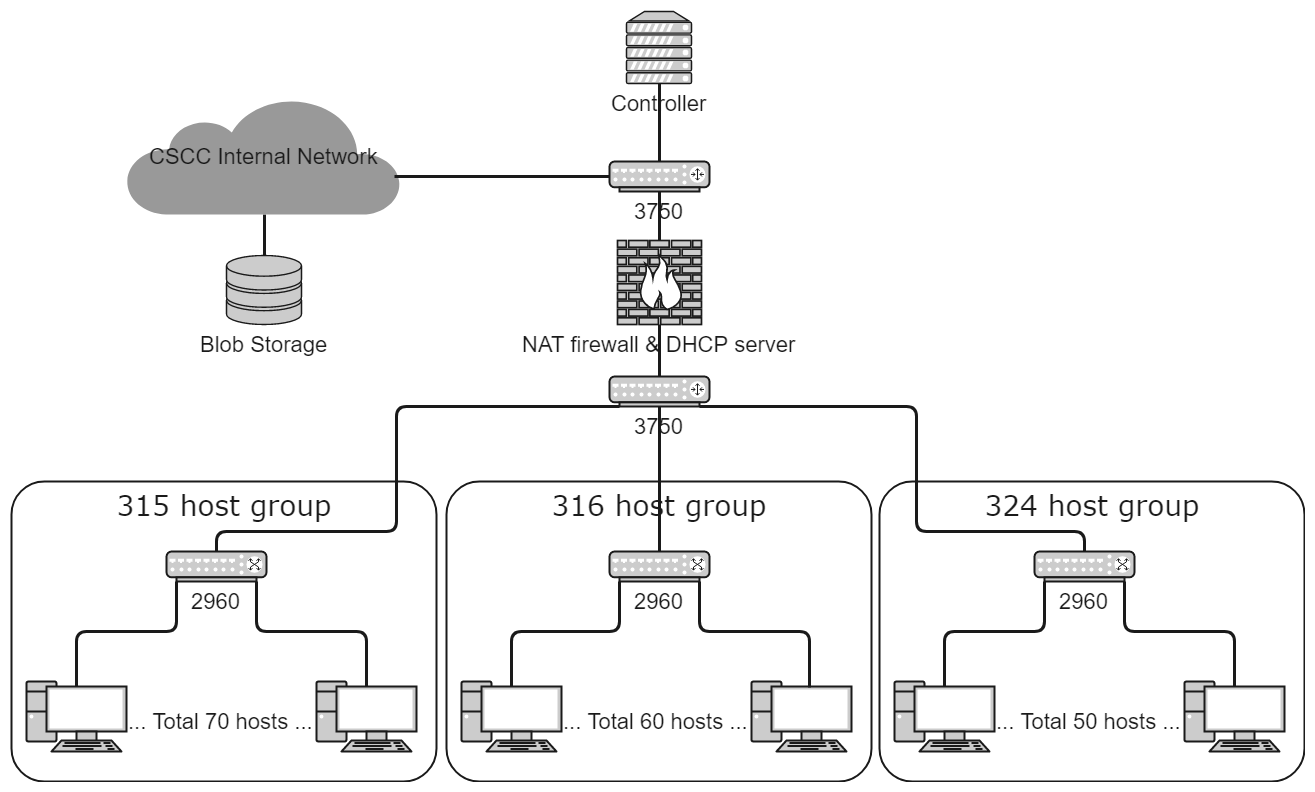
\includegraphics{images/PC_Room_Network.png}}
\caption{PC Room Network.}
\label{i:pcroom}
\end{figure}



*PC 電腦教室架構圖*
在交通大學資訊工程學系計算機中心,需要大量部屬 PC 電腦教室 Windows 環境與管理。從圖\ref{i:pcroom}可以看見計算機中心有三個主機群,主機數量分別為 50 台在 324 主機群、60 台在 316 主機群、70 台在 315 主機群。

由於 BitFission 目標主機群是 PC 電腦教室,因此將透過 Wake-On-Lan、PXE 和 Ansible,進行 Bare-Metal 操作與組態設定,即使沒有 IPMI 可以遠端操作的功能,BitFission 仍可以完成目標主機群的開關機與自動化部屬。
以下幾個步驟 映像檔產生 映像檔部屬 組態設定

\section{映像檔產生}
\subsection{Partclone}
Partclone 是一個工具程式來備份與還原分割區中的檔案資料,針對支援的檔案系統,只讀寫分割區有使用到的資要區塊(used blocks),其餘區塊就予以略去。透過這樣的方式,可以增加讀寫的效率,不需浪費時間與儲存空間來處理沒有使用的到區塊資料。支援ext2, ext3, ext4, reiserfs, reiser4, xfs, jfs, btrfs, FAT12, FAT16, FAT32, NTFS, HFS, UFS。*Partclone 映像檔 Layout*


\subsection{EZIO torrent}
*torrent 格式如何與硬碟 mapping*
在 Partclone 備份(Clone)過程中插入製作 Torrent 的程式碼,使得產生映像檔的過程中連帶計算 Torrent 所需要的 pieces checksum 、block offset 和 block size,省去重新讀取硬碟資料來製作 Torrent 的時間。

\subsection{SquashFS}
*TODO 用 Squashfs 進一步解決映像檔肥大問題*

\subsection{BitAtom}
\begin{figure}[!htbp]
\centering
\scalebox{.5}{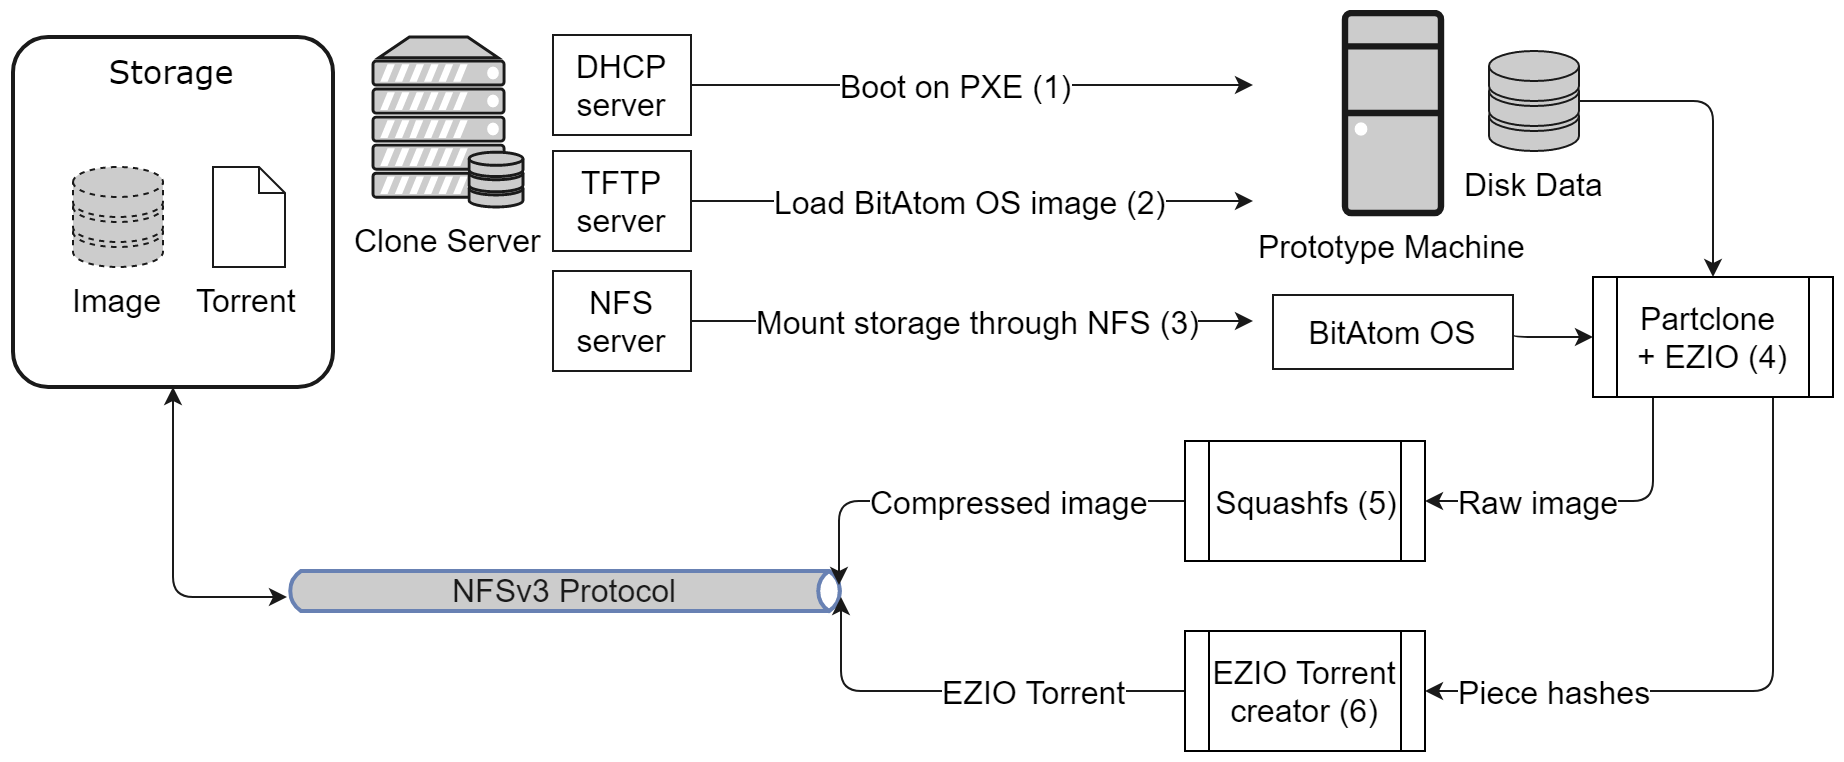
\includegraphics{images/BitAtom_Flowchart.png}}
\caption{BitAtom Flowchart.}
\label{i:bitatomflowchart}
\end{figure}



映像檔產生流程如圖\ref{i:bitatomflowchart}
為了自動化產生映像檔,本研究使用 archiso 客製化了自動備份的作業系統 BitAtom,BitAtom 包含 Partclone。透過 PXE 開機載入 BitAtom 作業系統映像檔,執行 Partclone 將原型機的檔案系統轉換成映像檔與 Torrent。
*可以透過ansible或是TFTP上設定的腳本自動產生映像檔*


\section{映像檔部屬}
\subsection{EZIO}
為了解決 Server-Client 一對一效能問題以及 Clonezilla Multicast 封包遺失所造成的不穩定,BitFission 使用了基於 BitTorrent 協議的 EZIO 作為映像檔部屬的解決方案。因為 BitTorrent 透過 P2P 讓部屬速度接近 Multicast ,在特定情況下甚至可以超過 Multicast。*需要實驗數據*

\subsection{BitTorrent Features}
且 BitTorrent 具備非同步的特性,部屬時不受單一主機異常而影響其他主機,異常主機也可以在一定時間內重新回到部屬作業中。*原理解釋*


此外,由於 BitTorrent 的 resume 功能,使得部屬作業得以僅還原硬碟與映像檔有差異的片段 ( pieces ),進行差異式部屬降低硬碟寫入次數與網路傳輸量。對於使用同一基礎映像檔 ( Base Image ) 產生的差異映像檔 ( Differential Image ),可以提高部屬效率並減少硬碟寫入次數。

\subsection{BitFission Deployment Server}
部屬伺服器使用 BitTorrent 協議分析映像檔製作 torrent ,並以部署伺服器作為 tracker 和第一個 seeder 透過 P2P 進行部屬。之後使用 Wake-On-LAN 喚醒目標主機群,以 PXE 開機載入 S. EZIO 系統。 S. EZIO 系統透過 BitTorrent 協議和 tracker 溝通後找到 seeder ,執行 EZIO 程式與 seeder 交換映像檔並寫入硬碟中完成映像檔部屬。

再生與還原流程如圖\ref{i:flowchart}。


\begin{figure}[!htbp]
\centering
\scalebox{.56}{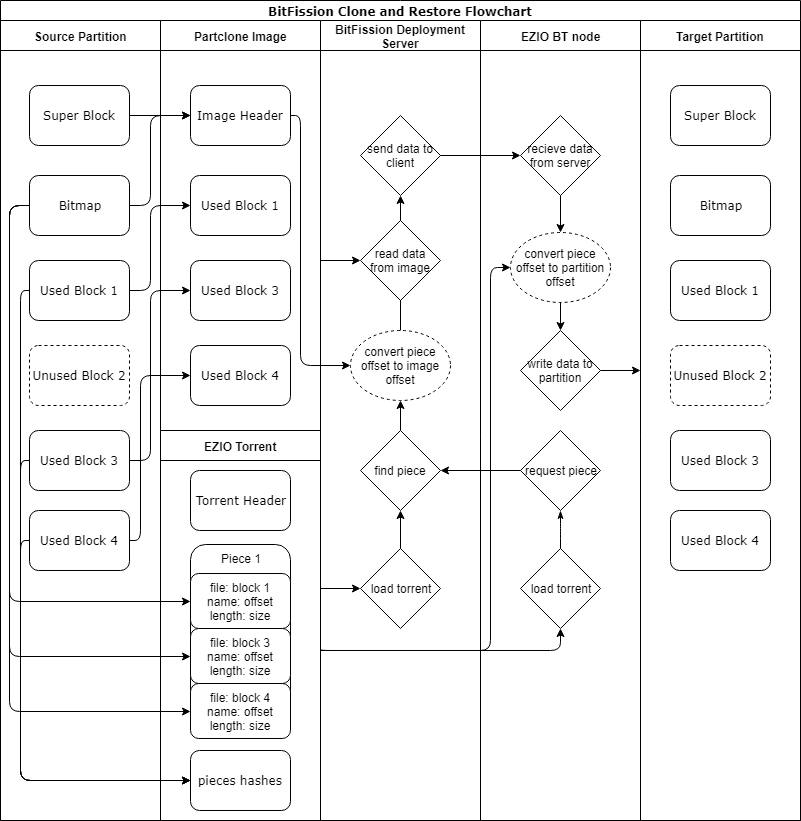
\includegraphics{images/BitFission_Clone_Flowchart.png}}
\caption{BitFission Flowchart.}
\label{i:flowchart}
\end{figure}



\section{組態設定}
\subsection{Ansible}
Ansible 是一個開原的組態管理工具,作為 BitFission 後續設定的解決方案。選用 Ansible 原因是由於 agentless 架構以及其連線機制是透過 ssh 或 winrt ,可以自由的整合不同作業系統,包含 Unix-like 和 Windows 作業系統。此外,Ansible 也不用在部屬時在映像檔加入憑證,如 Puppet 是透過憑證認證,每台主機必須事先產生不同憑證才能夠與 Puppet 進行後續設定。綜合以上優點,我們使用 Ansible 作為 Bare-Metal 主機群的組態管理工具。
映像檔部屬後所需的後續設定 ( Post-Configuration ) ,BitFission 採用 Ansible 調整每台主機的差異部分,例如修改主機名稱與加入 Active Directory 等等動作。以此架構達成自動化 Bare-Metal 機器部屬與服務開通 ( Provisioning )。
